\chapter{Data Streams}
\label{ch:DataStreams}

For those familiar with PHENIX software, data structures, and raw data
processing, this chapter may be skipped. However, as this note will eventually
be part of my thesis, I have gone into detail. For an executive summary list of
all data sources used in this analysis, I have provided it here:

\begin{itemize}
\item PRDF Data (available on either 1 second intervals, or event-by-event basis)
  \begin{itemize}
  \item GL1P-0: "BBCLL1(\textgreater0 tubes)"
  \item GL1P-1: "CLOCK"
  \item GL1P-2: "ZDCLL1Wide"
  \item GL1P-3: "ZDCLL1Narrow"
  \item event-sequence
  \item ATP number
  \item epoch time stamp
  \item GL1 crossing ID (bunch number)
  \end{itemize}
\item BPM Data (available in four second intervals)
  \begin{itemize}
  \item Sector 7 Blue Beam x position
  \item Sector 7 Blue Beam y position
  \item Sector 7 Yellow Beam x position
  \item Sector 7 Yellow Beam y position
  \item Sector 8 Blue Beam x position
  \item Sector 8 Blue Beam y position
  \item Sector 8 Yellow Beam x position
  \item Sector 8 Yellow Beam y position
  \item epoch time stamp
  \end{itemize}
\item WCM and DCCT Data (avaialble every few seconds)
  \begin{itemize}
  \item WCM population for each bunch
  \item DCCT beam current for blue beam
  \item DCCT beam current for yellow beam
  \item epoch time stamp associated with each field of WCM or DCCT data
  \end{itemize}
\item DST Data
  \begin{itemize}
  \item BbcOut Node
    \begin{itemize}
      \item BBC pmt tubes fired north
      \item BBC pmt tubes fired south
      \item BBC event z-vertex
    \end{itemize}
  \end{itemize}
  \begin{itemize}
  \item ZdcOut Node
    \begin{itemize}
      \item ZDC event z-vertex
    \end{itemize}
  \end{itemize}
  \begin{itemize}
  \item TrigLvl1 Node
    \begin{itemize}
      \item bitmasked triglive
      \item bitmasked trigscaled
      \item bitmasked trigraw
    \end{itemize}
  \end{itemize}  
  \begin{itemize}
  \item SpinDataEventOut Node
    \begin{itemize}
      \item GL1P crossing ID
      \item event-sequence
      \item GL1P-0: "BBCLL1(\textgreater0 tubes)"
      \item GL1P-1: "CLOCK"
      \item GL1P-2: "ZDCLL1Wide"
      \item GL1P-3: "ZDCLL1Narrow"
    \end{itemize}
  \end{itemize}  
\end{itemize}

The vernier analysis is unique among various PHENIX analyses because it requires
that data streams from RHIC machine sources and the PHENIX detector are
synchronized. It is also unique in that the data set itself exibits obvious time
dependent behavior. This introduces interesting challenges, as PHENIX software
generally does not provide tools to deal with time dependent data, and
synchronization of PHENIX data with other RHIC data streams is infrequently
done; PHENIX and RHIC data streams effectively live in entirely different
software universes (post data production), so there is no guarantee of a common
key which can be used to synchronize the data, once we have obtained it. 

Previous analyses have generally dealt with each data stream separately,
combining only when absolutely neccessary. This approach favors simplicity, but
is generally hard to generalize to any data set from any year. PHENIX data sets
are generally analyzed as a phase-space data set, with no desire to understand
or account for time dependant effects.  However, the vernier analysis is
intrinsically a time-dependent analysis, so it makes intuitive sense to do the
analysis in a way which mirrors the physical process of the vernier scan.

Unfortunately, this means that for portions of the analysis, one must resort to
using raw PHENIX data, which incidentally, is not too difficult, it just
requires a small amount of custom software to be written.

By understanding the data structures which are available, I have written
software (with huge thanks to Joe Seele and Martin Purschke for help with this)
which can generally cross check and reproduce any vernier analysis that has been
undertaken in previous years, and this has been exploited to provide fast
cross-check for the Run 15 vernier analysis. In fact, as it turns out, thanks to
the Common-Device (CDEV) data packet contained in PHENIX Raw Data Format files,
we can effectively do the analysis starting from the PRDF packet level to
achieve total data synchronization. This makes the process of synchronization
much easier, as well as reproducing the various data sets from raw data (if
avaialble) more straight forward. 

Some data is subject to correction for various systematic issues. Those
corrections are summarized in the Chapter~\ref{ch:SystematicCorrections}, but
are not discussed in detail here.

\section{Beam Position Monitors}
There are two beam position monitors BPM(s) located about 8 meters away from the
PHENIX IR on either side (BPM sector 7, and BPM sector 8). The BPMs may be used
to establish teh relative separation of the blue and yellow beams, but are not
good for establishing absolute beam position~\cite{Drees2013}.  The beam
position monitors are coupled capacitavely to the beam
pipe(Figure~\ref{fig:bpm_schematic_cartoon}), with pick ups on the left and
right of the pipe, and pickups above and below the pipe. Every four seconds,
data is read out from the BPMs. We are given an x and y position, plus an epoch
time stamp associated with the blue and yellow beams, from sector 7 and sector 8
respectively. We can geometrically extrapolate the intersection of the blue and
yellow beams respectively in the PHENIX IR plane, and then calculate the net
separation between the two beams, Figure
~\ref{fig:bpm_ir_xing_cartoon}.

The BPM data obtained contains measurements of beam position over the course of
an entire fill, containing a vernier scan. We use the start and end run times to
isolate a chunk of BPM data corresponding to the vernier scan. The data set
contains the following fields:
\begin{itemize}
\item epoch time
\item blue beam, sector 7 x position
\item blue beam, sector 7 x position
\item blue beam, sector 8 y position
\item blue beam, sector 8 y position
\item yellow beam, sector 7 x position
\item yellow beam, sector 7 x position
\item yellow beam, sector 8 y position
\item yellow beam, sector 8 y position
\end{itemize}

\begin{figure}[ht]
  \begin{center}
    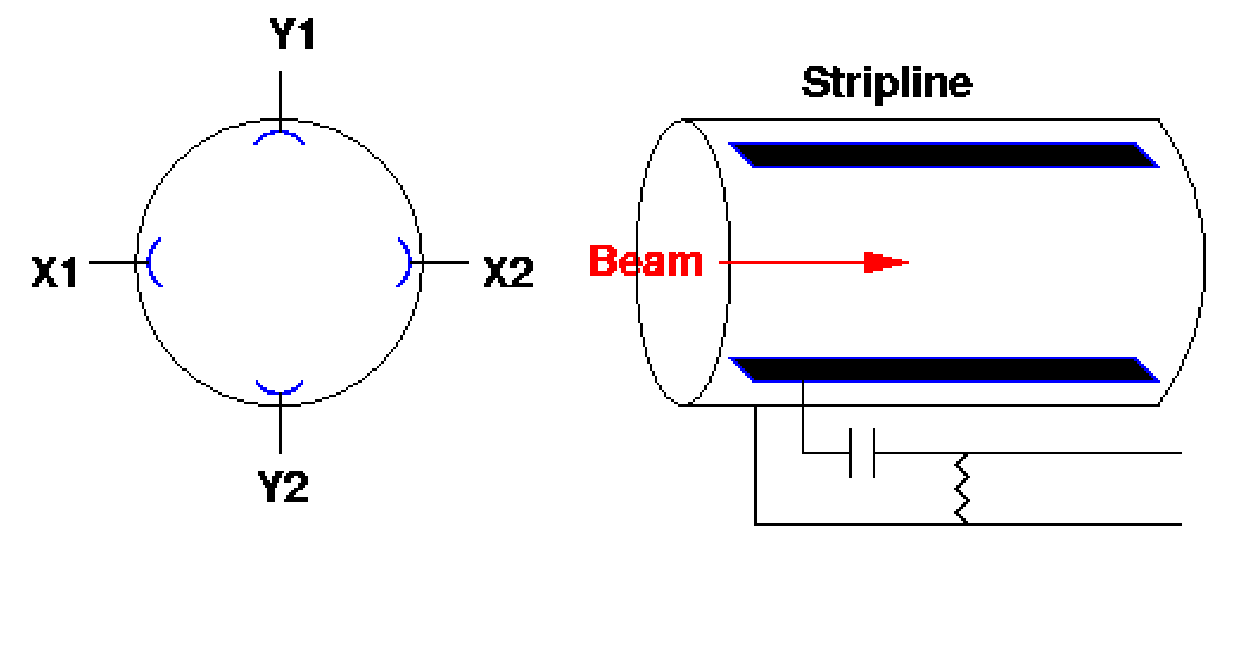
\includegraphics[width=1.0\linewidth]{./figures/bpm_schematic}
    \caption{ Beam Current induces a time dependent voltage proportional to the derivative of
      the beam current itself. BPM electronics use a comparator circuit, and the readings from
      X1/2 and Y1/2 to determine the X and Y beam positions. The absolute measurement of beam
      position is subject to offsets stemming from various effects, however, relative positions
    (say of one beam to another) are reliable.~\cite{kawallfocus2005}}
    \label{fig:bpm_schematic_cartoon}
  \end{center}
\end{figure}


\begin{figure}[ht]
\begin{center}
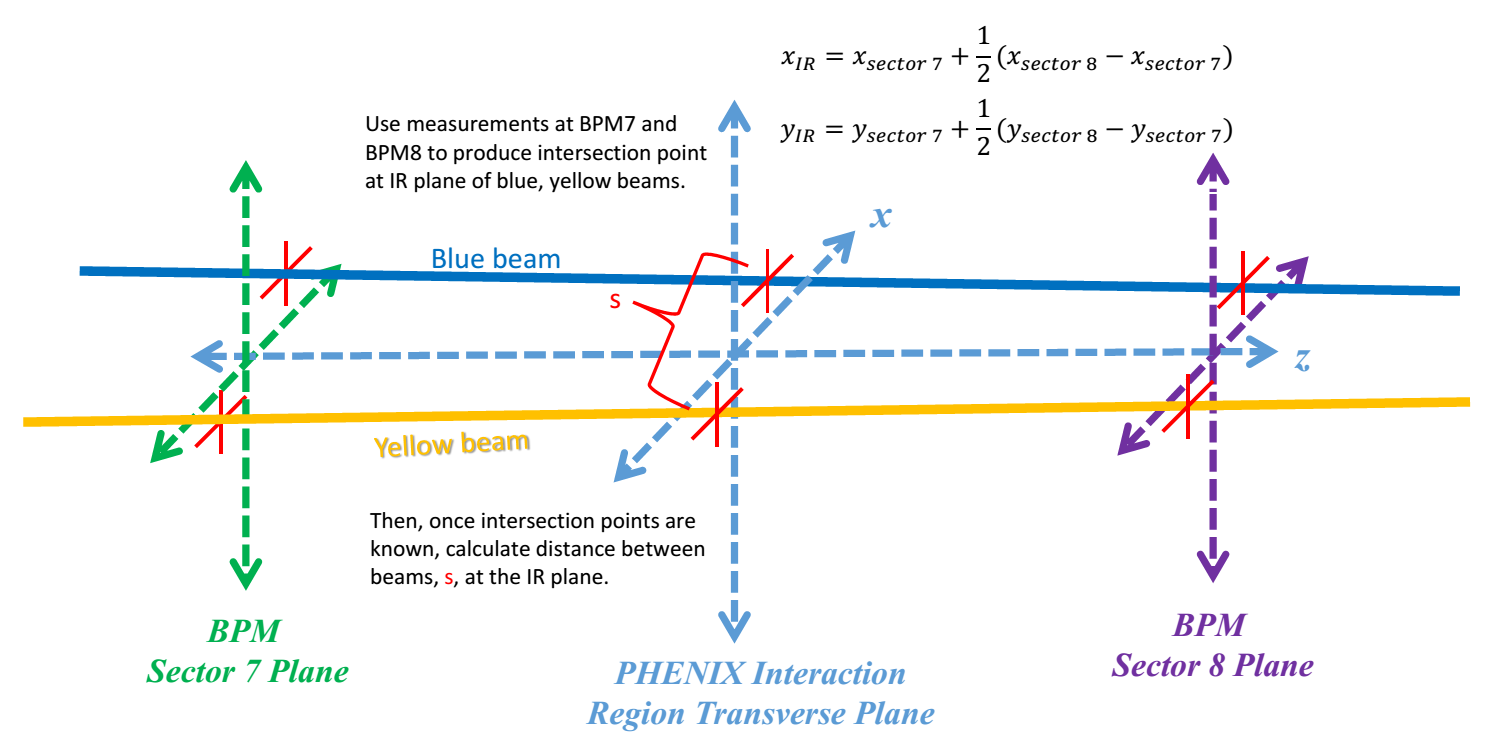
\includegraphics[width=1.0\linewidth]{./figures/bpm_ir_beam_separation}
\caption{We define three parallel planes, each plane is perpendicular to the beam axis.
The planes are at the Sector 7 BPM, the PHENIX IR, and Sector 8 BPM. We assume that the
two BPM planes are equidistant from the PHENIX IR. We can geometrically solve for a three
dimensional line intersecting all three planes, since we have access, for each beam,
intersection points for a given beam at Sector 7 and Sectro 8. With this information, we
determine the intersection points in the transverse plane in the PHENIX IR, and then use
the two intersection points at the IR plane of the blue and yellow beams to calculate
relative beam separation, in both horizontal and vertical directions.}
\label{fig:bpm_ir_xing_cartoon}
\end{center}
\end{figure}

\section{PHENIX Raw Data Format} 

The PHENIX raw data format (better known as PRDFs) are the form that recorded
data takes immediately after being assembled into events, by the PHENIX DAQ.
PRDF data is archived soon after being generated on the massive robotic tape
filesystem. PRDF data is hierarchichal, first being organized by event-type, and
then organized by packet-type.  Every packet has a header, which contains
general information such as what the packet contains, and in what order that
packet was recieved. Every packet recorded can be associated with a unique
event-sequence number, which specifies roughly the order in which the event
owning the packet was recieved by the DAQ. Within a given run number, an
event-number is guaranteed to be unique. The complexity of the packet is limited
by the bandwidth available to move data off PHENIX onto other storage, and the
buffers/reconstruction ability of the front end electronics modules built onto
PHENIX subsystems.

Generally, raw PHENIX data is too complex to use straight-away, because minimal
to no reconstruction of physical properties for a certain event is done (and
this varies by the subsystem, and hardware constraints of the subsystem).
However, for the vernier analysis, we are generally only interested in very,
very simple properties of an event, all of which are completely avaialble
directly from the PRDF. This allows us a huge flexibility, as other then the
libraries required to dump packet information from PRDFs (i.e. the Event.h)
headers, there are no dependancies for obtaining the data we need from PRDFs.

One constraint of using PRDFs as a primary data source is that disk space
becomes a constraint. A normal physics run may be segmented into hundreds of
PRDFs, each at 20 GB in size. However, because the event rates are on average,
quite low for a vernier scan, and because vernier scans typically do not last
longer than 20 minutes, there are typically only five or six PRDFs needed to
store an entire scan, but in general, using PRDF data without tested data
recustruction libraries requires careful checking of the final product.

The data extracted from PRDFs is summarized in table~\ref{tab:prdf_data_summary}.


\subsection{GL1-1P Scalers, ATP Numberand Event Time Stamps}
The DAQ supports 32 possible triggers, which may be designed to be arbitrarily
sensititve to arbitrary hardware signal coincidences. When PHENIX experiences a
trigger, all PHENIX detector subsystems dump the FEM buffers to a the sub-event
builders (SEB) which reconstruct raw events, and then pass these events along to
the ATPs (Assembly and Trigger Processor) to compress and assemble the events
into PRDFs. Over the course of this process, the event is categorized by event
type (here, we are concerned with "DATAEVENT" and "SCALEREVENT" types), tagged
with a number ($0 \leq ATPNUMBER < 64$), corresponding to the ATP which
processed the event, and given an epoch time-stamp. Since time is synchronized
between the ATPs via the network, there may be some latency, and these time
stamps must be corrected for an offset.  Because of the large volume of data,
several thousand events will arrive for processing simultaneously, so we can
simply choose an ATP (I choose "0") and correct all other time offsets of other
ATPs relative to this time, such that we obtain a time offset that we can use to
synchronize all epoch times to within one second accuracy for the entire data
set.

Other data that are extracted from PRDFS (besides ATPNUMBER, EPOCHTIME,
RUNNUMBER, and EVENTNUMBER) are BUNCHNUMBER, and the GL1-1P scalers.

GL1-1P Scalers are unique counters which may be programmed to track any
arbitrary trigger. These counters count the number of "live" triggers for each
programmed triggers which occur between recorded events. Each time an event is
recorded, the counter dumps the number of "in between" triggers to the GL1P
packet. For Run 12, the triggers programmed into the GL1-1P boards were:

\begin{itemize}
\item BOARD-ID: 0, "BBCLL1(\textgreater0 tubes)"
\item BOARD-ID: 1, "CLOCK"
\item BOARD-ID: 2, "ZDCLL1Wide"
\item BOARD-ID: 3, "ZDCLL1Narrow"
\end{itemize}

Generally, to obtain a rate for these trigger scalers, we have two options:
\begin{enumerate}
\item Sum all scalers associated with a single EPOCHTIME to get that scaler's per second
rate
\item Take the ratio of a particular scaler to the "CLOCK" scaler, converting to a rate
using the clock frequency ($9.36MHz$).
\end{enumerate}

Generally the two options should yield the same results, unless there are DAQ
issues related to live time. Since this is generally the case, item 2 is
generally the preferred method, though there are other methods for correcting
for live time. For example, one can use raw events counters, which are contained
in "SCALEREVENT" packets and find the ratio between those events and live events
contained in "SCALEREVENT" packets.
% need to format initial columns so that there is more room (can we wrap text in a
% header?)
\begin{sidewaystable}[ht]
\centering
\begin{tabular}{ l l p{6cm} p{8cm} }
\toprule
\textbf{Source} & \textbf{Field} & \textbf{Description} & \textbf{Application} \\
\midrule 
Event Header & EPOCHTIME & Standard unix time & Time ordering data, Calculation of real-time GL1-1P scaler rates \\
 & ATPNUMBER & ID for ATP handling this event & Synchronization of EPOCHTIME for all events \\
 & RUNNUMBER & Standard PHENIX run ordering & \\
 & EVENTNUMBER & Unique identifier showing order in which DAQ processed events & Unique sorting key, proxy for time \\
Packet 140008 & GL1-1P 0 & "BBCLL1(\textgreater0 tubes)" & Counts live events between recorded events \\
 & GL1-1P 1 & "CLOCK" & "" \\
 & GL1-1P 2 & "ZDCLL1Wide" & "" \\
 & GL1-1P 3 & "ZDCLL1Narrow" & "" \\
Packet 140001 & Gl1-Crossing ID & Identify bunch crossing  & Used to track beam width, $\sigma_{BBC}$  for specific bunches\\
\bottomrule
\end{tabular}
\caption{ Data extracted from PRDFs. }
\label{tab:prdf_data_summary}
\end{sidewaystable}

\subsection{Scaler Events}
Scaler events are a special type of event which tracks the total number of times
each one of the 32 triggers has fired. These counters are naturally extremely
large numbers, and are avaialble for access in scaler events which are produced
once every four seconds.  Using these counters can be useful for calculating
live time, as we get both live trigger sums and raw trigger sums for all 32
bits. These scalers are used in the Run Control Log to generate overall
statistics for each PHENIX run, but many don't realize that we have nearly
real-time access to these coutners at the PRDF level.

\section{Data Summary Tape}
Data Summary Tapes (more commonly referred to as DSTs) are reconstructed data
files generated from PRDFs. They are one of the several filetypes generated when
PRDFs-events are reconstructed and/or processed. Generally, these files are
simply ROOT files which contain trees, historgrams, or specialized classes used
to serialize and organize data.  The primary advantage of using DSTs is that the
file size is small relative to PRDFs, and that there is some amount of
consistancy in the way that all DSTs are produced. DSTs are often further
reduced to simple ntuples, via Fun4All. The PHENIX Fun4All data reconstruction
framework also handles the reduction of PRDFs to other data agglomerations.

The vernier analysis uses its own special data production, and uses the
following analysis
nodes (Tabel~\ref{tab:dstnodes}).

Rates have been extracted and cross checked against rates which are found in
PRDFs, and they are identical. The analysis currently only uses the DSTs for
calculation of the BBC efficinecy. This will likely not change, because we want
to calculate the efficiency of various flavors of minimum bias triggers in this
analysis, and this requires that we look at other runs, which contain hundreds
of segments. 

\begin{table}
  \centering
  \begin{tabular}{ l p{6cm} }
    \toprule
    \textbf{Node} & \textbf{Description} \\
    \midrule 
    BbcOut           & Number of north/south photomultiplier tubes fired, and BBC event z-vertex \\
    ZdcOut           & Zdc event z-vertex  \\
    TrigLvl1         & Bitmask for live-events, raw-events and scaled-events. \\
    SpinDataEventOut & Event-sequence, gl1crossing ID (bunch number), four gl1-1p scalers \\
    \bottomrule
  \end{tabular}
  \caption{ A brief summary of data-nodes which are used in the vernier analysis, via DST }
  \label{tab:dstnodes}
\end{table}

\section{Wall Current Monitor and Direct-Current Current-Transformer}
The wall current monitor and direct-current current-transformers (WCM and DCCT,
respectively) allow us to use induced image-charges in plates capacitively
coupled to beam current to calculate the total number of ions in the blue and
yellow beams (most accurately using DCCT) and determine individual bunch
populations (WCM). Since the DCCT is more accurate, it can be used to calibrate
the overall values of bunch populations after summation.

Like the BPM data, WCM and DCCT data can be in principal accessed from the CDEV
packet in PRDFs, however, the framework for doing this has not been developed,
as the data streams were parsed from log files and data bases at the time of the
various vernier scans.

\begin{figure}[ht]
  \begin{center}
    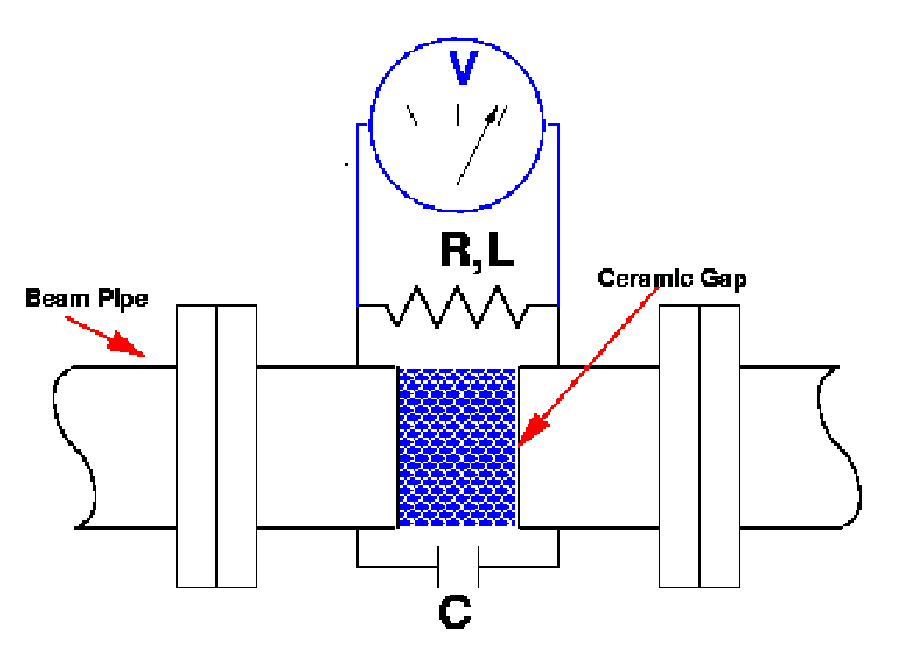
\includegraphics[width=0.75\linewidth]{./figures/wcm_schematic_cartoon}
    \caption{ 
      Here we see an insulating ceramic break in the beam pipe, which shunts
      image wall currents from the beam pipe around the toriud. Magnetic
      shielding excludes external magnetic fields.~\cite{kawallfocus2005} 
    }
    \label{fig:wcm_schematic_cartoon}
  \end{center}
\end{figure}

\begin{figure}[ht]
  \begin{center}
    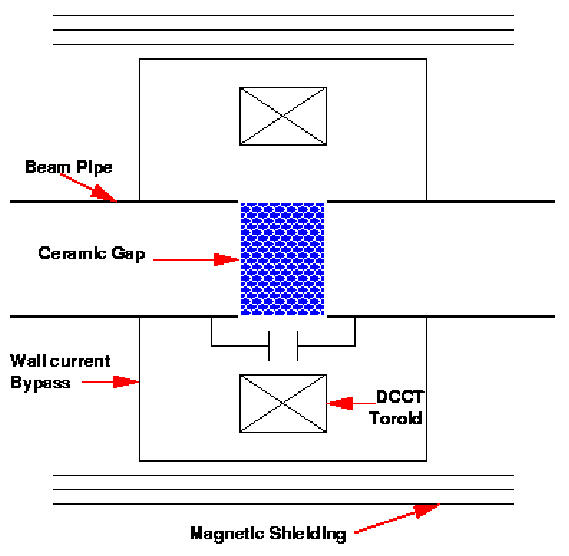
\includegraphics[width=0.75\linewidth]{./figures/dcct_schematic_cartoon}
    \caption{
      The wall current monitor uses an insulating ceramic break in the beam pipe
      similarly to the DCCT, which forces image wall currents through
      electronics which measure the current frequencies. The WCM is sensitive
      only to bunched beams, and can measure longitudianl profiles of bunches
      ~\cite{kawallfocus2005}.
    }
    \label{fig:dcct_schematic_cartoon}
  \end{center}
\end{figure}

\section{Software Repositories}
I've developed a suite of software tools which deal with various data streams
and analysis segments. The code is extensively documented, so I show its
location in CVS here using broad strokes.

I use the PHENIX CVS repository to contain my vernier analysis code. All of my
vernier analysis code can be found at: offline/analysis/beaumim/vernierScan .

Relative to this repository root, I have roughly subdivided the other
repositories within this root according to the basic tasks it handles.

\begin{itemize}
\item vernier\_analysis
  \begin{itemize}
    \item Uses output from vernier\_DST\_reduction as input
    \item Beam Width
    \item BBC Rate Calculation
    \item BPM Data Visualization
    \item BBC Efficiency
    \item Parameterization of Vernier Scan Steps
  \end{itemize}
\item prdf\_analysis
  \begin{itemize}
    \item prdf\_tools/full\_prdf\_scalers
      \begin{itemize}
        \item Dumps gl1p, bunch, atp and time stamp from PRDF to text file
	\item corrects time stamp
	\item merges PRDF dumps into single file
	\item projects prdf data dumps into bunch integrated, and bunch separated data
	sets, summed down to indivudual time stamps
      \end{itemize}
    \item prdf\_tools/scalers
      \begin{itemize}
        \item Reads a PRDF and dumps raw and live scalgger scalers relevant to the vernier
	analysis. Does scaler overflow corrections.
      \end{itemize}
    \item prdf\_tools/processing
      \begin{itemize}
        \item Processes BBC Rates
	\item Processes Beam Position
	\item Beam Width
      \end{itemize}
  \end{itemize}
\item vernier\_DST\_reduction
  \begin{itemize}
    \item Reads DSTs and outputs root files with histograms and tree
   \end{itemize}
\end{itemize}
